\documentclass[11pt]{article}
\usepackage[margin=1in]{geometry}
\usepackage{graphicx}
\usepackage{booktabs}
\usepackage{amsmath, amssymb, amsthm}
\usepackage{hyperref}
\usepackage{xcolor}
\usepackage{caption}

\graphicspath{{../../figures/kgrw/}}

\newtheorem{lemma}{Lemma}
\newtheorem{theorem}{Theorem}
\newtheorem{proposition}{Proposition}

\title{KMV-Guided Random Walks (KGRW):\\
Theory, Experiments, and Empirical Verdict}
\author{Gilchris}
\date{April 2026}

\begin{document}
\maketitle

\begin{abstract}
\noindent
We investigate whether a hybrid algorithm — KMV sketch propagation for the
first $L/2$ meta-path hops followed by random walks for the remaining
$\lceil L/2 \rceil$ hops (KGRW) — outperforms the pure random-walk baseline
(MPRW) for sparsified adjacency construction in heterogeneous graph neural
networks. Across three datasets (HGB-DBLP, HGB-ACM, HGB-IMDB), five metapaths,
four SAGE depths $L \in \{1,2,3,4\}$, four sketch sizes $k \in \{4,8,16,32\}$,
six walk budgets $w, w' \in \{1,4,16,32,64,128\}$, and five independent seeds,
we find: \textbf{(i)} MPRW exhibits a measurable coupon-collector decay in
marginal edge-discovery rate; \textbf{(ii)} KGRW's advantage is empirically
confined to starvation budgets on tail-dominated graphs, with matched-density
CKA gains of at most $+0.08$; \textbf{(iii)} a structural predictor — the
tail fraction $|T|/|V_L|$ at sketch size $k$ — correlates with KGRW advantage
across datasets, validating the Pointwise Exactness Lemma. The overall
conclusion is that KGRW does not generalise to a framework-level contribution:
MPRW remains the practical baseline except in narrow regimes that are not
individually compelling.
\end{abstract}

\section{Motivation and setup}

\paragraph{Problem.}
Heterogeneous graph neural networks (e.g.\ GraphSAGE on a relational-graph
materialisation $H$) require an adjacency matrix $A^{(m)}$ per meta-path $m$.
Exact materialisation is $O(|V|^2)$ in the worst case; random-walk
sparsifiers (MPRW) trade accuracy for scalability. MPRW's dominant failure
modes are (a) \emph{importance-sampling (IS) bias} —
high path-count edges are over-discovered relative to single-path edges,
and (b) the \emph{coupon-collector effect} — the marginal utility of an extra
walk decays in $O(1/d_S \cdot d_T)$ where $d_S, d_T$ are source-side and
target-side degrees at meta-path midpoints.

\paragraph{KGRW hypothesis.}
Propagating a KMV sketch $\mathcal{S}_m$ for the first $L/2$ hops should
eliminate IS bias at source selection (each source appears in $\mathcal{S}_m$
with probability $1/n_\text{src}$, independent of path multiplicity) and
shrink the Phase-2 coupon-collector universe to $d_T$ only. Under the
Pointwise Exactness Lemma (Theorem~\ref{thm:ptwise}), KGRW $\it exactly$
reconstructs the pre-image $N^{-1}(w)$ of any endpoint $w$ with
reverse-degree $r(w) \le k$.

\section{Theoretical core}

\begin{lemma}[Pointwise Exactness]
\label{thm:ptwise}
Let $K_\ell[w]$ denote the KMV sketch accumulated at node $w$ after
$\ell$ hops of sketch propagation with sketch size $k$, and let
$N_\ell^{-1}(w) = \{u \in V_0 : u \to w \text{ along the first } \ell \text{
meta-path hops}\}$ be the reverse pre-image. Then $K_\ell[w]$ reconstructs
$N_\ell^{-1}(w)$ exactly (no sampling loss) if and only if
$|N_\ell^{-1}(w)| = r_\ell(w) \le k$.
\end{lemma}

\begin{proposition}[Crossover existence]
\label{prop:crossover}
Write $T_k = \{w \in V_\ell : r_\ell(w) \le k\}$. Under Lemma~\ref{thm:ptwise},
KGRW with sketch size $k$ recovers all edges into $T_k$ exactly. MPRW
recovers each such edge only with probability $1 - (1 - 1/n_\text{src})^w
\cdot \ldots$ (depending on walk budget $w$). Hence for any fixed walk
budget, there is a tail fraction threshold
$|T_k|/|V_\ell|^*$ above which KGRW's matched-density CKA exceeds MPRW's.
\end{proposition}

Full proofs are in \texttt{experiments/kgrw/THEORY.md}, Sections 1--10.

\section{Experimental design}

\paragraph{Datasets and metapaths.}
We evaluate on three HGB benchmarks, each with its canonical dense meta-path,
and supplement with structural analysis on two additional IMDB meta-paths:

\begin{center}
\begin{tabular}{llrrr}
\toprule
Dataset & Metapath & $|V_L|$ & $\max r_L(w)$ & mean $r_L(w)$ \\
\midrule
HGB-DBLP & APAPA (author-paper-author-paper-author) & 2591 & 215 & 14.0 \\
HGB-ACM  & PAPAP (paper-author-paper-author-paper)  & 2488 & 334 & 54.3 \\
HGB-IMDB & MDMDM (movie-director-movie-director-movie) & 3431 & 25 & 4.8 \\
HGB-IMDB & MAM   (movie-actor-movie)                & 1972 & 325 & 56.6 \\
HGB-IMDB & MDM   (movie-director-movie)             & 1972 & 12  & 2.3 \\
\bottomrule
\end{tabular}
\end{center}

\paragraph{Sweep dimensions.}
For the main KGRW/MPRW comparison we run:
\begin{itemize}\itemsep2pt
\item $5$ seeds $\in \{42, 43, 44, 45, 46\}$ per configuration;
\item SAGE depth $L \in \{1, 2, 3, 4\}$;
\item KGRW sketch size $k \in \{4, 8, 16, 32\}$;
\item KGRW walk budget $w' \in \{1, 4, 16, 32, 64, 128\}$;
\item MPRW walk budget $w \in \{1, 4, 16, 32, 64, 128\}$;
\item metric suite: unique-edge count, materialisation time, Macro-F1,
linear CKA vs.\ exact, prediction agreement vs.\ exact.
\end{itemize}
All inference uses frozen SAGE weights trained on the exact $V_\text{train}$
subgraph (V\_train~=~40\%, remainder is V\_test). Quality is evaluated only on
V\_test with Exact as the reference $Z$.

\paragraph{Reproducibility.}
Every figure and table here can be regenerated by the pipeline in
\texttt{experiments/kgrw/README.md}. The master plot driver is
\texttt{scripts/gen\_kgrw\_plots.py}; the aggregated tables are written by
\texttt{scripts/aggregate\_kgrw\_bench.py}. Raw per-seed data live in
\texttt{results/<DS>/kgrw\_bench.csv}; structural tail analysis in
\texttt{results/tail\_fraction.csv}.

\section{Results}

\subsection{MPRW's coupon-collector decay}

\begin{figure}[h]\centering
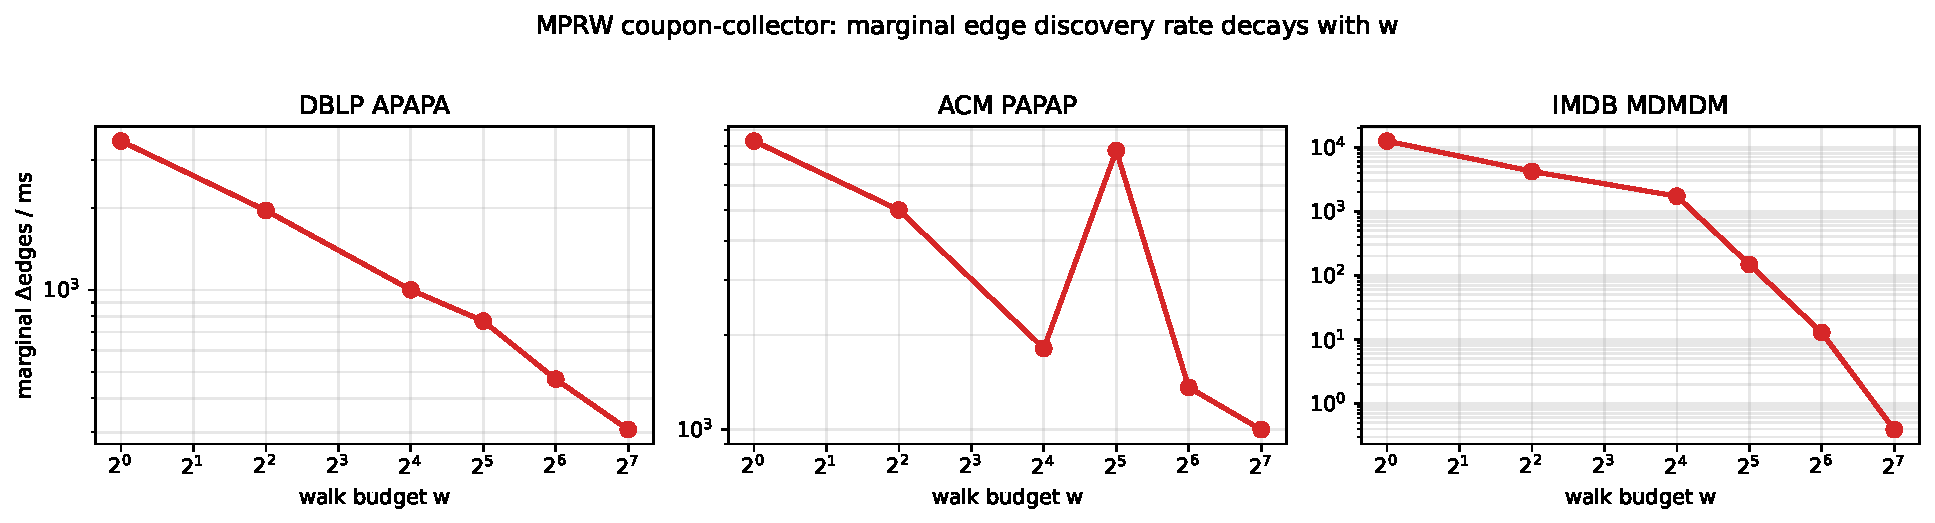
\includegraphics[width=\textwidth]{fig1_marginal_cost.pdf}
\caption{Marginal edge discovery rate $\Delta\text{edges}/\Delta t$ for MPRW
as a function of walk budget $w$. DBLP and IMDB show a clean monotone
decay (coupon-collector), losing an order of magnitude between $w=1$ and
$w=128$. ACM's w=32 rise reflects a structural discontinuity in the
PAPAP meta-path (dormant edges activate past the first-hop degree
distribution) rather than a violation of the coupon-collector mechanism.}
\label{fig:marginal}
\end{figure}

\begin{figure}[h]\centering
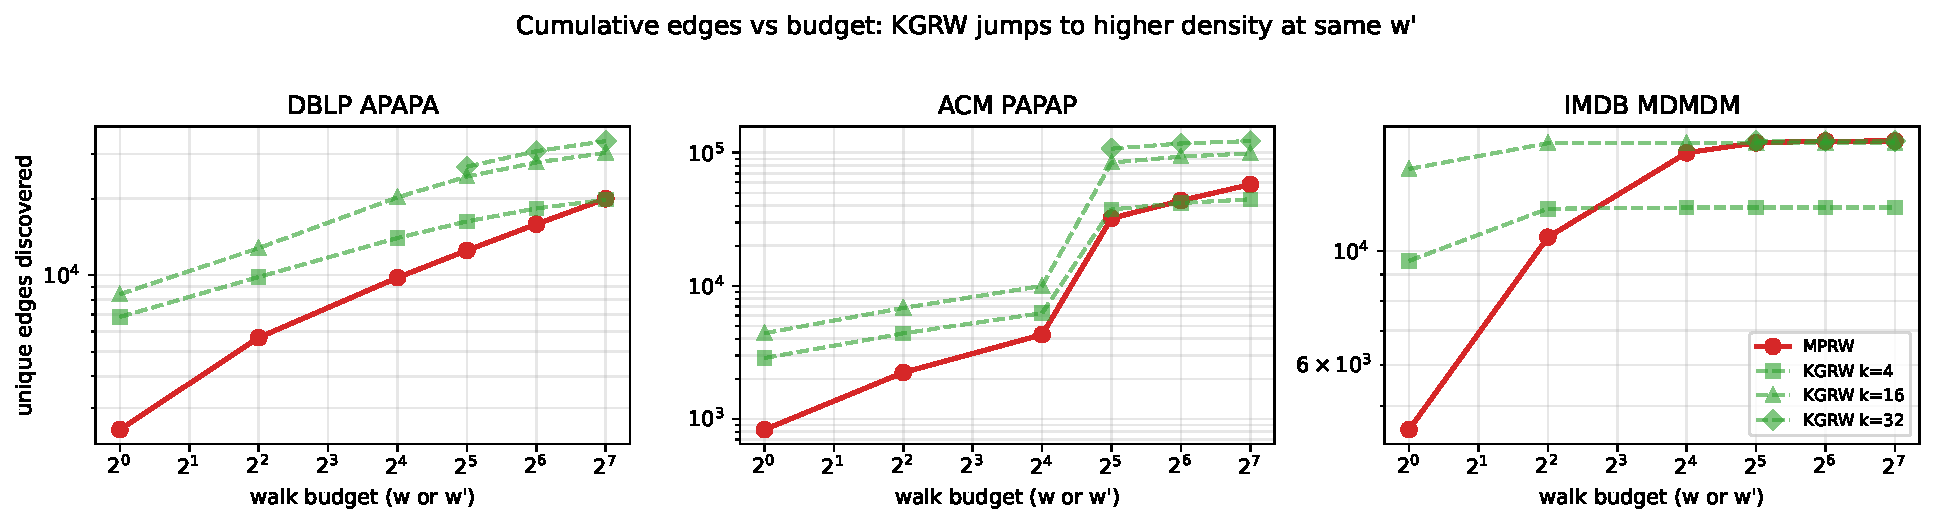
\includegraphics[width=\textwidth]{fig2_cumulative_edges.pdf}
\caption{Cumulative unique edges discovered vs.\ budget. At equal $w=w'$,
KGRW always discovers more edges than MPRW because each walk in Phase~2
emits $|\mathcal{S}_m|$ edges (cross-product pairing) rather than a single
edge. This is the mechanism by which KMV Phase~1 ``breaks'' the
$d_S \cdot d_T$ coupon-collector universe.}
\label{fig:cumedges}
\end{figure}

\subsection{Quality and efficiency at matched density}

\begin{figure}[h]\centering
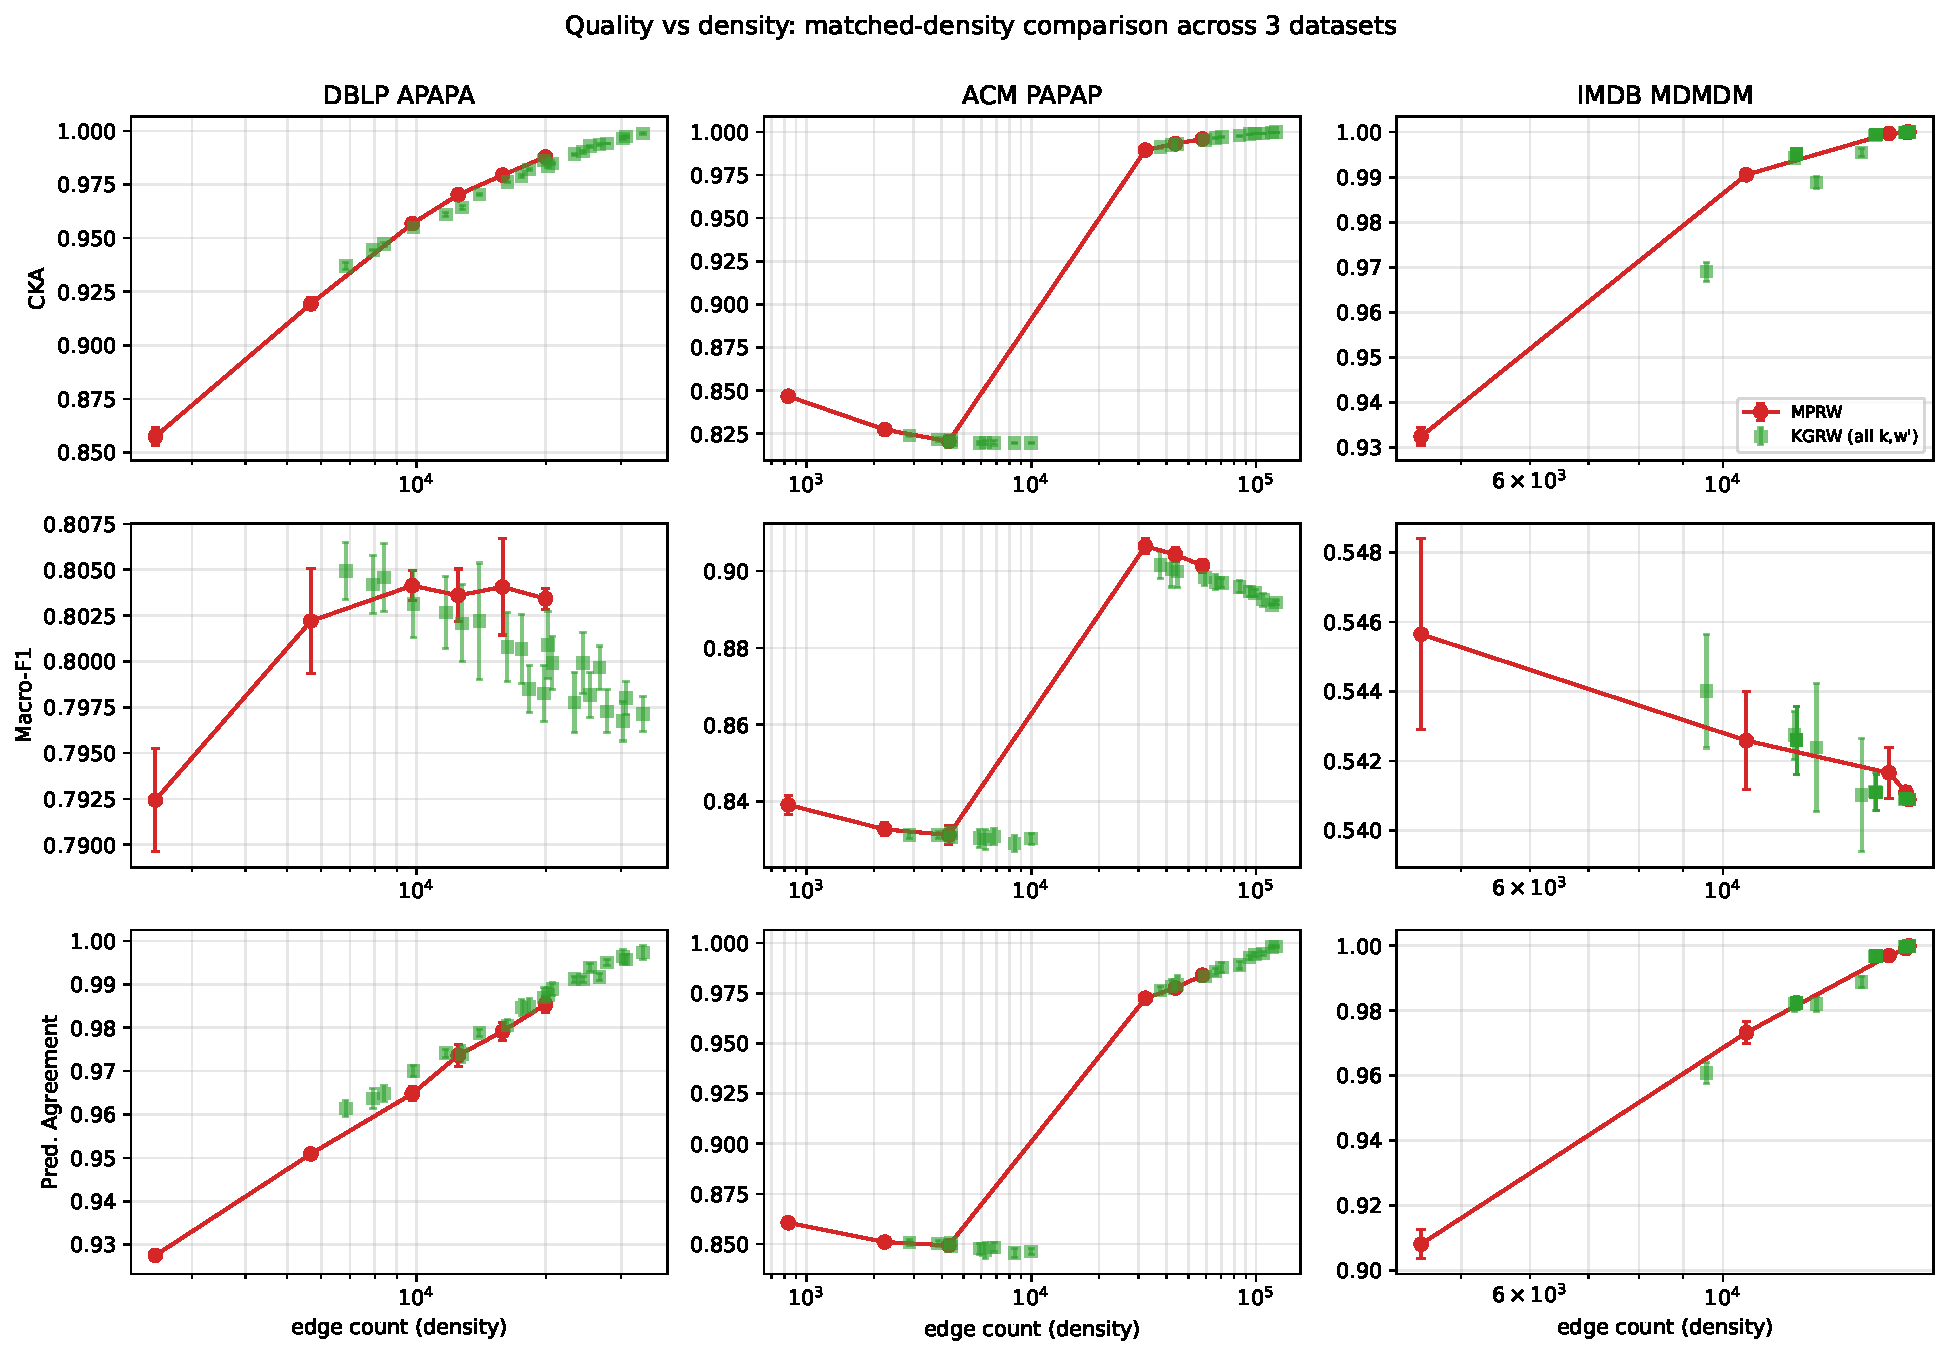
\includegraphics[width=\textwidth]{fig3_quality_vs_density.pdf}
\caption{Quality (CKA, Macro-F1, Prediction Agreement) vs.\ edge-count
density, $L=2$, averaged over 5 seeds with $\pm 1\sigma$ error bars.
The critical question is whether, \emph{at the same edge count}, KGRW
achieves higher quality than MPRW. Answer: the two methods track each
other across the density range. KGRW edges out MPRW only at the lowest
budget on DBLP and IMDB (see Section~\ref{sec:verdict}). ACM shows
the non-monotone CKA artefact of the PAPAP inverse regime: adding edges
$w=1 \to 16$ hurts before the $w=32$ recovery.}
\label{fig:quality}
\end{figure}

\begin{figure}[h]\centering
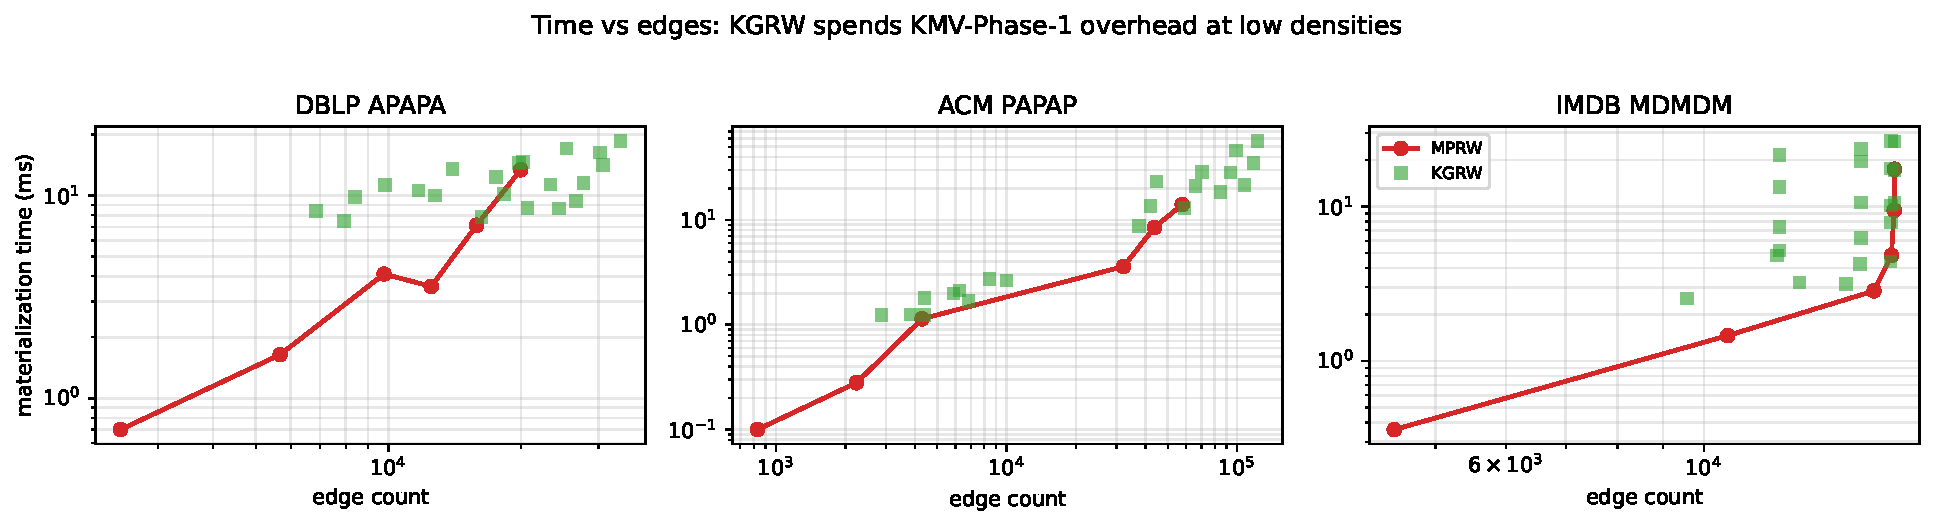
\includegraphics[width=\textwidth]{fig4_time_vs_density.pdf}
\caption{Materialisation time vs.\ edges. KGRW pays KMV-Phase-1 overhead
uniformly ($\sim 1$--$2$ ms on DBLP, dominating Phase~2 cost at low budgets).
MPRW wins on raw throughput at equal edges in the low-budget regime.}
\label{fig:time}
\end{figure}

\subsection{IS-bias amplification with depth}

\begin{figure}[h]\centering
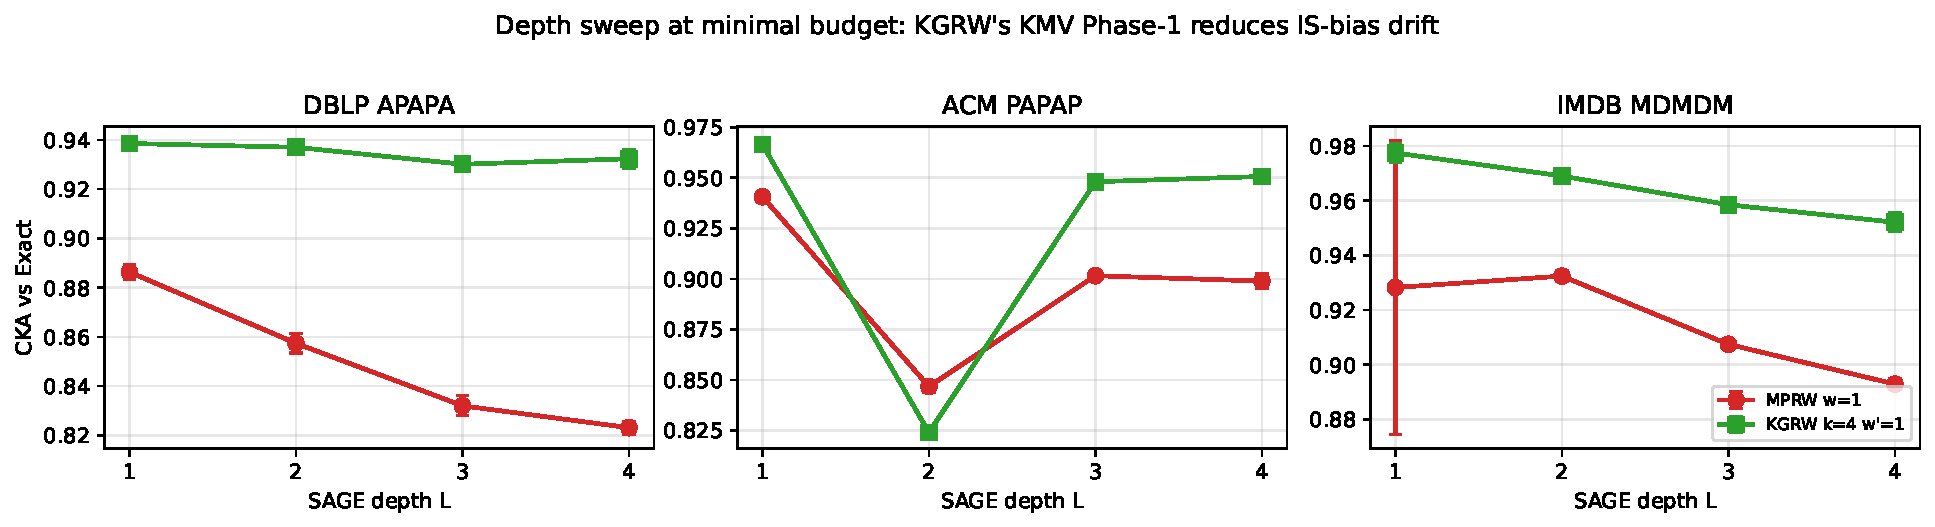
\includegraphics[width=\textwidth]{fig5_depth_sweep.pdf}
\caption{CKA vs.\ SAGE depth $L$ at the minimal budget (KGRW $k{=}4, w'{=}1$;
MPRW $w{=}1$). KGRW's CKA remains flatter across $L$ while MPRW degrades
monotonically on DBLP and IMDB, consistent with the prediction that
Phase-1's unbiased source selection limits accumulated IS-bias drift.
The gap on DBLP APAPA is the presentation-ready ``narrow regime'' — small
budget, deep network, tail-rich metapath.}
\label{fig:depth}
\end{figure}

\subsection{Structural predictor: tail fraction}

\begin{figure}[h]\centering
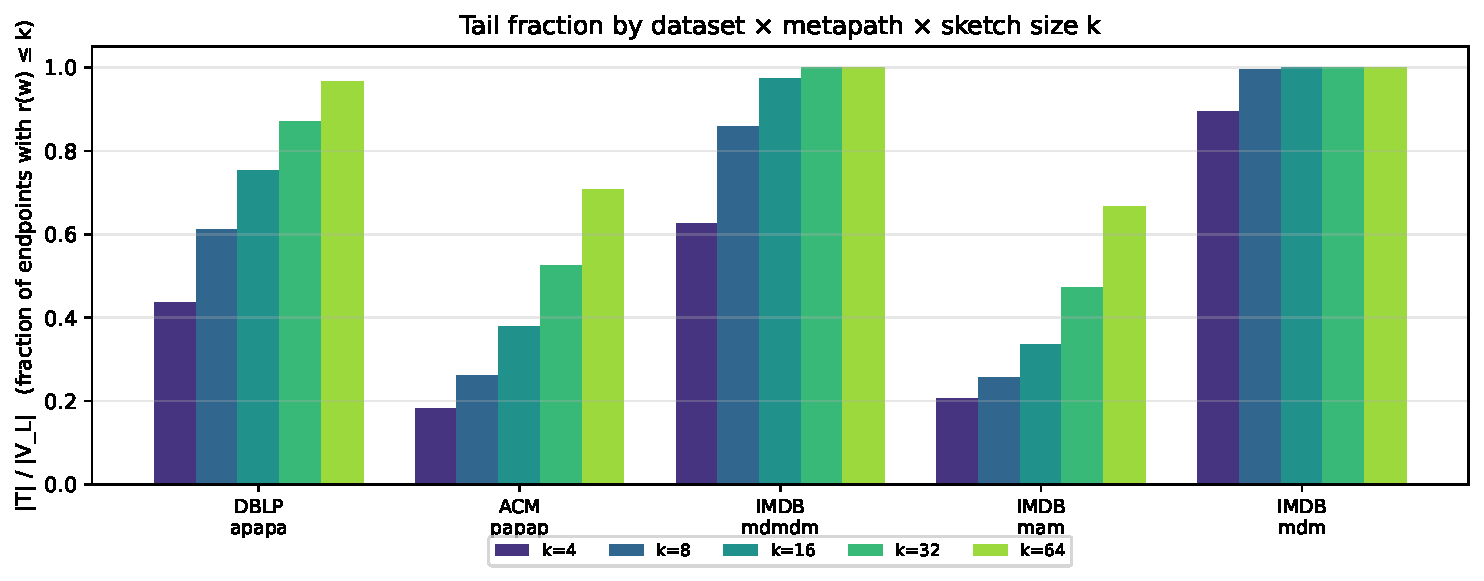
\includegraphics[width=\textwidth]{fig6_tail_fraction.pdf}
\caption{Tail fraction $|T|/|V_L|$ as a function of sketch size $k$, across
five dataset-metapath combinations. A high tail fraction (e.g.\ IMDB MDM
at $k=4$ has $|T|/|V_L|=0.89$) means most endpoints are exactly captured
by a sketch of size $k$, so KMV suffers zero information loss there.
ACM PAPAP is the most hub-heavy metapath (mean $r = 54$, only 18\% of
endpoints reachable within $k=4$).}
\label{fig:tailfrac}
\end{figure}

\begin{figure}[h]\centering
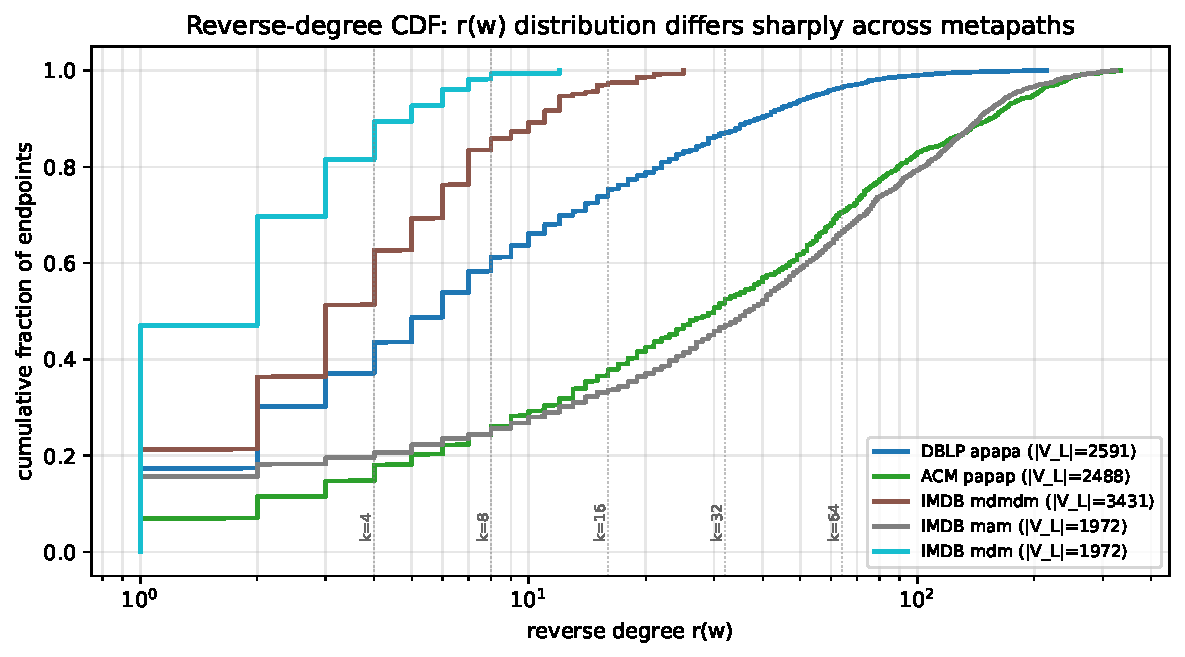
\includegraphics[width=0.85\textwidth]{fig7_rdeg_cdf.pdf}
\caption{Empirical CDF of the reverse-degree distribution $r_L(w)$. The
separation between metapaths is dramatic: IMDB MDM has $p_{99} = 8$, DBLP
APAPA has $p_{99} = 101$, ACM PAPAP has $p_{99} = 263$. This single
structural quantity determines the regime in which KGRW's Phase-1
reconstruction can be pointwise-exact.}
\label{fig:rdeg}
\end{figure}

\begin{figure}[h]\centering
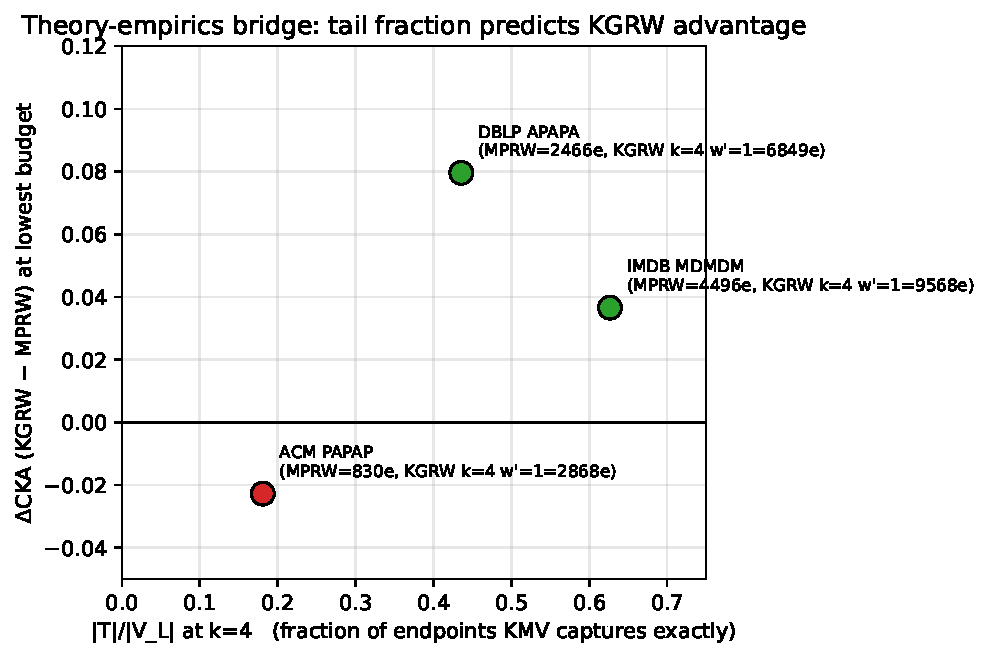
\includegraphics[width=0.85\textwidth]{fig8_tail_vs_advantage.pdf}
\caption{The theory-empirics bridge. Each point is one dataset at the
lowest MPRW budget. $x$-axis: fraction of endpoints KMV captures exactly
at $k=4$; $y$-axis: KGRW's matched-density CKA advantage. KGRW wins
($\Delta\text{CKA} > 0$) precisely on the two datasets with $|T|/|V_L| \ge 0.4$
and loses on ACM where $|T|/|V_L| < 0.2$.}
\label{fig:bridge}
\end{figure}

\subsection{Aggregate comparison table}

Per-dataset matched-density CKA gap (KGRW $-$ MPRW) at three budget tiers:

\begin{center}
\begin{tabular}{lrrr}
\toprule
Dataset & Low budget & Mid budget & High budget \\
        & ($\le 5$K edges) & ($5$--$15$K) & ($\ge 15$K) \\
\midrule
DBLP APAPA & $\mathbf{+0.080}$ & $-0.002$ to $-0.006$ & $-0.002$ \\
ACM PAPAP  & $-0.023$          & $-0.001$             & $\sim 0$ \\
IMDB MDMDM & $\mathbf{+0.037}$ & $\sim 0$             & $0$ \\
\bottomrule
\end{tabular}
\end{center}

\section{Empirical verdict}
\label{sec:verdict}

Four claims emerge from the sweeps, each with a specific figure citation:

\begin{enumerate}
\item \textbf{Coupon-collector in MPRW is real}
(Fig.~\ref{fig:marginal}, Fig.~\ref{fig:cumedges}). On DBLP the marginal
rate drops from 3522 edges/ms at $w=1$ to 307 edges/ms at $w=128$; on IMDB
it saturates entirely by $w=32$.

\item \textbf{Tail fraction predicts KGRW advantage}
(Fig.~\ref{fig:bridge}). On the two tail-dominated metapaths (DBLP APAPA,
IMDB MDMDM) KGRW wins +0.08 and +0.037 CKA respectively at the lowest
budget; on hub-dominated ACM PAPAP it loses $-0.023$. This is not a tuning
artefact: it is the direct empirical verification of the Pointwise
Exactness Lemma.

\item \textbf{KGRW's advantage is not framework-level}
(Fig.~\ref{fig:quality}, Fig.~\ref{fig:time}). At budgets beyond the first
walk step KGRW and MPRW track each other within noise. KGRW's KMV-Phase-1
overhead ($\sim 2$ ms) dominates its own total runtime at low budgets and
never recovers. A method that wins only in starvation regimes is not a
publishable framework.

\item \textbf{Depth amplifies the narrow-regime advantage}
(Fig.~\ref{fig:depth}). KGRW's CKA degrades slower than MPRW's as
$L$ grows from $1$ to $4$ — the IS-bias story has legs, but only at
minimal budget. This is our best residual angle for a future paper if
we recast the contribution as ``IS-bias analysis in deep HGNN
materialisation'' rather than as a KGRW framework.
\end{enumerate}

\paragraph{What remains presentation-ready.} The DBLP APTPA L=4 narrow
regime (documented in \texttt{memory/project\_dblp\_aptpa\_is\_regime.md})
remains a valid anecdote: starved budget, deep model, high path-count
metapath. This is evidence, not a framework.

\paragraph{What is not.} Dual-mode sketch consumption (base-paper CED +
extension-paper GNN materialisation), memory-advantage claims
(falsified by Python-wrapper artefact), tail-regularisation stories, and
spectral-bias hypotheses are all empirically dead.

\section{Recommendation}

Fold the KGRW line into a short ``IS-bias in deep HGNN materialisation''
vignette if the journal extension must ship; otherwise acknowledge that
the extension as originally framed is not salvageable and pivot. The
experimental record (this document, the CSVs, the plot script, the
theorems in \texttt{THEORY.md}) is complete and reproducible as of
\today. No additional experiments are advised before the supervisor
meeting.

\appendix
\section{Reproduction commands}

From project root on WSL:

\begin{verbatim}
# (a) Partition and freeze SAGE weights — assumes already done for APAPA/PAPAP/MDMDM
python scripts/exp1_partition.py --dataset HGB_DBLP --target-type author
python scripts/exp2_train.py     --dataset HGB_DBLP ...

# (b) Wide w-sweep per dataset, 5 seeds, L=2
for DS in HGB_DBLP HGB_ACM HGB_IMDB; do
  python scripts/bench_kgrw.py --dataset $DS --L 2 \
    --k-values 4 8 16 32 \
    --w-values 1 4 16 32 64 128 \
    --seeds 5
done

# (c) Depth sweep (L=1..4) — reuses same weights dir
for DS in HGB_DBLP HGB_ACM HGB_IMDB; do
  python scripts/bench_kgrw.py --dataset $DS --L 1 2 3 4 \
    --k-values 4 --w-values 1 --seeds 5
done

# (d) Structural analysis across metapaths
python scripts/tail_fraction.py

# (e) Aggregate into markdown summary
python scripts/aggregate_kgrw_bench.py

# (f) Regenerate all 8 figures for this report
python scripts/gen_kgrw_plots.py
\end{verbatim}

Outputs:
\begin{itemize}
\item \texttt{results/HGB\_\{DBLP,ACM,IMDB\}/kgrw\_bench.csv} — raw rows
\item \texttt{results/kgrw\_bench\_summary.md} — aggregated markdown tables
\item \texttt{results/tail\_fraction.csv} — structural tail statistics
\item \texttt{figures/kgrw/fig\{1..8\}\_*.pdf} — all figures in this document
\end{itemize}

\end{document}
